%!TEX root = practicum1.tex
\begin{figure}
	\centering
	\begin{subfigure}[b]{0.3\textwidth}
		\centering
		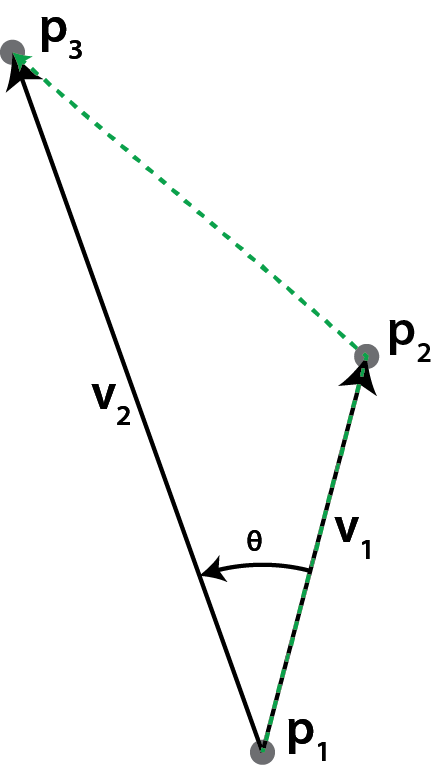
\includegraphics[width=0.9\textwidth]{./img/b_LeftTurn.png}
		\caption{left turn}
		\label{subfig:b:LeftTurn}
	\end{subfigure}
	\begin{subfigure}[b]{0.3\textwidth}
		\centering
		\includegraphics[width=0.9\textwidth]{./img/b_rightTurn}
		\caption{right turn}
		\label{subfig:b:RightTurn}
	\end{subfigure}	
	\begin{subfigure}[b]{0.3\textwidth}
		\centering
		\includegraphics[width=0.9\textwidth]{./img/b_noTurn}
		\caption{no turn}
		\label{subfig:b:NoTurn}
	\end{subfigure}		
	\caption{A path, the green dashed line, through the points $\vec{P_1}$, \vec{P_2} and \vec{P_3} making (\subref{subfig:b:LeftTurn}) a left, (\subref{subfig:b:RightTurn}) a right turn and (\subref{subfig:b:NoTurn}) no turn.}
	\label{fig:b:turns}
\end{figure}

\autoref{fig:b:turns} presents the three possible types of paths that form a straight line through the points $\vec{P_1}$, $\vec{P_2}$ and $\vec{P_3}$. Converting these three 2D points to three dimensional ones, by adding a $z$-coordinate that is zero, allows us to use the cross product to determine the angle $\theta$, using the definition of the cross product:

\begin{equation}\label{eq:b:crossProduct}
	\vec{v_1} \times \vec{v_2} = 
	\norm{\vec{v_1}} \cdot \norm{\vec{v_2}} \cdot \vec{n} \cdot \sin \theta.
\end{equation}
Where the $\vec{v_1} = \vec{P_2} - \vec{P_1}$, $\vec{v_2} = \vec{P_3} - \vec{P_1}$ and $\vec{n} = [0, 0, 1]$ represents the normal of the plane that contains the points. 

Since all values but the last of the vector \vec{n} are zero the result of \eqref{eq:b:crossProduct} will be of the form $[0, 0, q]$, where $q$ is influenced by $\sin \theta$. The norms of the vectors \v{1} and \v{2} are greater than or equal to zero by definition. And does not influence the value of $q$. From this we can conclude that the sign, or the lack thereof of $q$ is completely dependent upon $\sin \theta$. As we are only interested in the direction of the angle, not in its size we can use this to determine the type of path.\\

If the points are collinear the angle $\theta$ is $\pi$ and which results in $q = 0$. If $q$ is negative the path makes a left turn, if $q$ is positive the path makes a right turn.\\

Using Mathematica, see \autoref{lst:b:mat}, we get an expression for the value of $q$:
\begin{equation}
	q = -\p{1}_y \p{2}_x + \p{1}_x \p{2}_y + \p{1}_y \p{3}_x - \p{2}_y \p{3}_x - \p{1}_x \p{3}_y + \p{2}_x \p{3}_y,
\end{equation}
where $\p{1}_y$ represents the $y$-coordinate of the point \p{1}.

\begin{lstlisting}[float, language=Mathematica, label={lst:b:mat}, caption={Mathematica code used to compute the value of $q$.}]
p1 = {p1x, p1y, 0};
p2 = {p2x, p2y, 0};
p3 = {p3x, p3y, 0};

v1 = p2 - p1;
v2 = p3 - p2;

Cross[v1, v2]	
\end{lstlisting}

% To determine the type of turn, if any, a path makes we are interested in the sign of angle $\theta$, shown in \autoref{fig:b:turns}, for both a left turn (\protect\ref{subfig:b:LeftTurn}) and a right turn (\protect\ref{subfig:b:RightTurn}). Each point $\vec{P_r}$ represents the vector $[x_r, y_r]$, with $r \in \{1, 2, 3\}$. Representing each point $\vec{P_3}$ as a three-dimensional vector results in the vector $[x_r, y_r, 0]$. The vector $\vec{v_1}$ is defined as $\vec{P_2} - \vec{P_1}$ and $\vec{v_2} = \vec{P_3} - \vec{P_1}$.

% Now that we have these definitions we can use the equality in \eqref{eq:b:crossProduct} to determine the sign of $\theta$, which should tell us if the line through the points $\vec{P_1}$, $\vec{P_2}$, and $\vec{P_3}$ makes a left or a right turn, or no turn at all. 

% The vector $\vec{n}$ is the unit normal vector of the plane of the vectors $\vec{v_1}$ and $\vec{v_2}$, since all points lie in the $z$-plane $\vec{n} = [0, 0, 1]$. We use $\vec{q} = [a, b, c]$ to denote the result of the cross product of the vectors $\vec{v_1}$ and $\vec{v_2}$. Since the first two elements of the vector $\vec{n}$ are zero, $a$ and $b$ are also zero.

% The scalars $\norm{\vec{v_1}}$ and $\norm{\vec{v_2}}$ are by definition positive, as is the one provided by the normal vector. Thus only the factor $\sin \theta$ influences the sign of $c$.





